% SC4013 --- Chapter 2: Authentication, Sessions, MFA and OAuth (0->100)
\chapter{Authentication, Sessions and Delegated Trust}\label{ch:auth}

\begin{quote}
\emph{``Who are you?''} and \emph{``Prove it''} are two different questions. Authentication answers both, and every web feature that follows depends on getting the answer right.
\end{quote}

\noindent\fbox{\parbox{\dimexpr\linewidth-2\fboxsep-2\fboxrule}{%
\textbf{From zero: no prior auth knowledge assumed.} We start from a locked diary and a bouncer checking wristbands, then build passwords, sessions, multi-factor and delegated login (OAuth) from first principles. Each mechanism is defined, its failure mode shown, and the fix motivated before any formalism.}}
\vspace{0.4em}

\section*{Learning Outcomes}
After this chapter you will be able to:
\begin{enumerate}[label=(L\arabic*)]
    \item distinguish identification, authentication, and authorisation;
    \item explain why passwords must be hashed with salt, pepper and a slow KDF;
    \item manage sessions securely (cookie flags, fixation, timeout);
    \item compare MFA factors and TOTP/WebAuthn trade-offs;
    \item trace the OAuth 2.0 + OIDC authorization-code flow and name its key threats.
\end{enumerate}

% ============================================================
\section{Who Are You? Identification versus Authentication}\label{sec:auth-basics}
Identification is claiming an identity (``I am \texttt{alice@example.com}''). Authentication is proving it. Authorisation---whether Alice may do something---comes \emph{after} we are sure who she is (Ch.~4).

Passwords remain the most common authenticator because they are cheap and familiar. The naive design is to store them verbatim and compare on login. That makes the database a treasure chest: one read (SQL injection, backup leak, rogue admin) compromises every account, especially since people reuse passwords across sites.

\begin{definition}[Password hashing requirements]\label{def:pw}
Store not $p$ but $h=KDF(p\parallel s)$ where $s$ is a unique random \emph{salt} per user and $KDF$ is deliberately \emph{slow} (bcrypt, scrypt, Argon2). The hash must be one-way, salt must be random per record, and iteration cost must be tunable so verification takes $\approx 100$--$500$~ms even as hardware improves.
\end{definition}

Why each piece matters: \emph{salt} defeats precomputed rainbow tables---identical passwords produce different hashes. \emph{Slow KDF} defeats brute force---an attacker who steals the table must spend milliseconds per guess rather than nanoseconds (MD5/SHA-256 are fast hashes, not password hashes). \emph{Pepper} (an application-wide secret stored outside the DB, e.g., in an HSM) means a DB dump alone is insufficient.

A quick cost argument: a GPU can try $\sim 10^{9}$ SHA-256 hashes per second but only $\sim 10^{2}$ bcrypt verifications per second at cost 12. For an 8-character alphanumeric password ($62^{8}\approx 2\times10^{14}$ guesses), SHA-256 falls in days, bcrypt in millennia. That is why ``fast hash + salt'' is still broken.

\begin{lstlisting}[language=Python]
# WRONG: fast hash, no salt -- cracked in seconds with rainbow tables
import hashlib
def check_login_bad(stored_sha256, password):
    return hashlib.sha256(password.encode()).hexdigest() == stored_sha256

# RIGHT: slow KDF with per-user salt (bcrypt) + pepper
import bcrypt, os
pepper = os.environ["PEPPER"]  # 32 random bytes, not in DB
def hash_password(pw: str) -> bytes:
    salted = (pw + pepper).encode()
    return bcrypt.hashpw(salted, bcrypt.gensalt(rounds=12))  # ~250 ms

def verify(stored: bytes, pw: str) -> bool:
    return bcrypt.checkpw((pw + pepper).encode(), stored)
\end{lstlisting}

Never cap password length at a small value, never email passwords in clear, and always rate-limit login attempts (e.g., 5 tries then exponential back-off) to blunt online guessing---but rate limits do not fix a leaked table of fast hashes. NIST SP 800-63B now recommends checking new passwords against known-breach corpora (e.g., Have I Been Pwned) and favouring length over complexity rules.

% ============================================================
\section{Sessions: Remembering Who You Authenticated}\label{sec:sessions}
HTTP is stateless. After the password check succeeds, the server must give the browser a \emph{session token} (usually a random string in a cookie) that says ``this bearer already proved they are Alice until time $T$.'' The token is a temporary credential and must be handled with the same care as a password. Two common forms are \emph{opaque tokens} (random ID looked up server-side, as below) and \emph{JWTs} (self-contained signed assertions); both need the same cookie discipline.

\begin{figure}[h]\centering
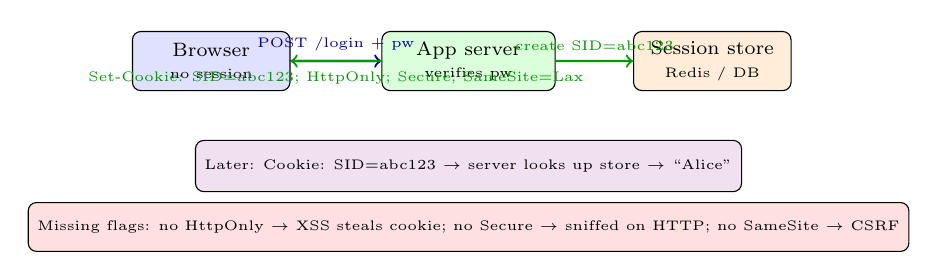
\begin{tikzpicture}[scale=0.86, every node/.style={font=\scriptsize}]
  \node[draw,fill=blue!12,rounded corners=3pt,minimum width=2.0cm,minimum height=0.75cm,align=center] (browser) at (-3.8,1.0) {Browser\\ \tiny no session};
  \node[draw,fill=green!14,rounded corners=3pt,minimum width=2.2cm,minimum height=0.75cm,align=center] (server) at (0,1.0) {App server\\ \tiny verifies pw};
  \node[draw,fill=orange!15,rounded corners=3pt,minimum width=2.0cm,minimum height=0.75cm,align=center] (store) at (3.6,1.0) {Session store\\ \tiny Redis / DB};
  \draw[->,thick,blue!60!black] (browser) -- (server) node[midway,above,font=\tiny] {POST /login + pw};
  \draw[->,thick,green!60!black] (server) -- (store) node[midway,above,font=\tiny] {create SID=abc123};
  \draw[->,thick,green!60!black] (server) -- (browser) node[midway,below,font=\tiny] {Set-Cookie: SID=abc123; HttpOnly; Secure; SameSite=Lax};
  \node[draw,fill=violet!12,rounded corners=3pt,minimum width=4.8cm,minimum height=0.65cm,align=center,font=\tiny] at (0,-0.55) {Later: Cookie: SID=abc123 $\to$ server looks up store $\to$ ``Alice''};
  % bad vs good cookie flags
  \node[draw,fill=red!12,rounded corners=3pt,minimum width=5.2cm,minimum height=0.62cm,align=center,font=\tiny] at (0,-1.45) {Missing flags: no HttpOnly $\to$ XSS steals cookie; no Secure $\to$ sniffed on HTTP; no SameSite $\to$ CSRF};
\end{tikzpicture}
\caption{Login $\to$ session establishment. The password is checked once; thereafter the random session ID (SID) is the credential. Cookie flags determine whether the browser will expose it to JavaScript, non-TLS links, or cross-site requests.}
\label{fig:session-flow}
\end{figure}

Secure cookie hygiene (all three matter): \texttt{HttpOnly} blocks \texttt{document.cookie} reads (mitigates XSS theft), \texttt{Secure} ensures the browser only sends it over HTTPS, and \texttt{SameSite=Lax/Strict} blocks cross-site POSTs (mitigates CSRF). The server should also rotate the SID on privilege change (login, password reset) to prevent \emph{session fixation}, set an idle timeout (15--30~min) and an absolute lifetime (8--24~h), and invalidate the old SID on logout. Use \texttt{\_\_Host-} prefix to bind the cookie to the host and path.

\begin{center}
\small
\begin{tabular}{lll}
\toprule
Attribute & What it does & Failure if omitted\\
\midrule
\texttt{HttpOnly} & Hides cookie from \texttt{document.cookie} & XSS exfiltrates SID directly\\
\texttt{Secure} & Only over HTTPS & SID sniffed on HTTP / captive portal\\
\texttt{SameSite=Lax} & Blocks cross-site POST & CSRF forges state-changing requests\\
\texttt{\_\_Host-} prefix & Binds to host, requires Secure + path=/ & Subdomain sets sibling cookie\\
\bottomrule
\end{tabular}
\end{center}

A classic \emph{session fixation} attack: (1) attacker visits site and gets SID=\texttt{attacker123}; (2) attacker tricks victim into using that SID (e.g., \texttt{https://site/login?SID=attacker123}); (3) victim logs in, server associates Alice with \texttt{attacker123} without rotation; (4) attacker now reuses the same SID to impersonate Alice. Rotation on login breaks step~(3).

JWTs as sessions deserve caution: a JWT in \texttt{localStorage} is readable by XSS, and revocation is hard because the token is self-validating until expiry. Prefer opaque SIDs in \texttt{HttpOnly} cookies; if you use JWTs, keep lifetimes short (minutes), store them in cookies, and maintain a denylist or rotation. For mobile apps, store refresh tokens in the OS keychain, not in clear files.

\begin{lstlisting}[language=Python]
# Flask-ish: setting session cookie securely
from flask import Flask, make_response
import secrets
app = Flask(__name__)
@app.route("/login", methods=["POST"])
def login():
    # ... verify password with bcrypt (above) ...
    sid = secrets.token_urlsafe(32)          # 256-bit random
    store.save(sid, {"user":"alice","exp": 3600})
    resp = make_response("ok")
    resp.set_cookie("SID", sid, httponly=True, secure=True,
                    samesite="Lax", max_age=3600, path="/")
    return resp

# On every authenticated request:
#  user = store.lookup(request.cookies.get("SID"))  # None -> 401
\end{lstlisting}

\begin{figure}[h]\centering
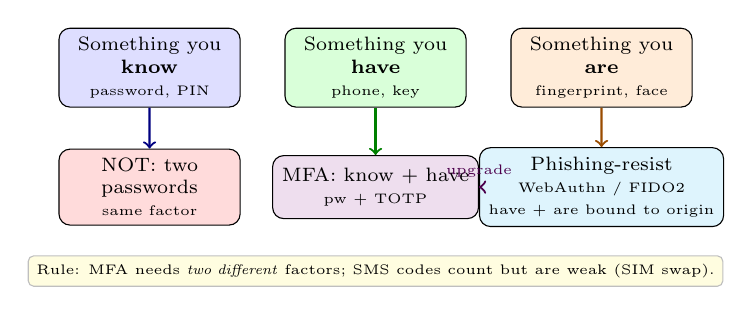
\begin{tikzpicture}[scale=0.82, every node/.style={font=\scriptsize}]
  \node[draw,fill=blue!13,rounded corners=4pt,minimum width=2.3cm,minimum height=0.8cm,align=center] (what) at (-3.5,1.3) {Something you\\ \textbf{know}\\ \tiny password, PIN};
  \node[draw,fill=green!15,rounded corners=4pt,minimum width=2.3cm,minimum height=0.8cm,align=center] (have) at (0,1.3) {Something you\\ \textbf{have}\\ \tiny phone, key};
  \node[draw,fill=orange!15,rounded corners=4pt,minimum width=2.3cm,minimum height=0.8cm,align=center] (are) at (3.5,1.3) {Something you\\ \textbf{are}\\ \tiny fingerprint, face};
  \node[draw,fill=red!14,rounded corners=4pt,minimum width=2.3cm,minimum height=0.8cm,align=center] (bad) at (-3.5,-0.55) {NOT: two\\ passwords\\ \tiny same factor};
  \node[draw,fill=violet!13,rounded corners=4pt,minimum width=2.3cm,minimum height=0.8cm,align=center] (good) at (0,-0.55) {MFA: know + have\\ \tiny pw + TOTP};
  \node[draw,fill=cyan!13,rounded corners=4pt,minimum width=2.3cm,minimum height=0.8cm,align=center] (best) at (3.5,-0.55) {Phishing-resist\\ \tiny WebAuthn / FIDO2\\ \tiny have + are bound to origin};
  \draw[->,thick,blue!50!black] (what) -- (bad); \draw[->,thick,green!50!black] (have) -- (good);
  \draw[->,thick,orange!60!black] (are) -- (best);
  \draw[->,thick,violet!60!black] (good) -- (best) node[midway,above,font=\tiny,sloped] {upgrade};
  \node[font=\tiny,fill=yellow!12,draw=gray!50,rounded corners=2pt,inner sep=3pt] at (0,-1.85) {Rule: MFA needs \emph{two different} factors; SMS codes count but are weak (SIM swap).};
\end{tikzpicture}
\caption{MFA factor taxonomy. Colour encodes factor type; the red box is the common mistake of stacking two ``know'' factors. The progression is toward origin-bound, phishing-resistant authenticators (FIDO2/WebAuthn) where the browser proves possession of a private key tied to the site's origin.}
\label{fig:mfa-factors}
\end{figure}

% ============================================================
\section{Multi-Factor and Passwordless}\label{sec:mfa}
A single factor fails in one step. \emph{Multi-factor authentication} (MFA) requires two \emph{different} factors so one breach does not suffice. The intuition is a safe-deposit box that needs both your key and the bank's key---stealing one is not enough.

\emph{TOTP} (RFC~6238, the 6-digit codes from Authenticator apps) mixes a shared secret with the current 30-second window: $\text{code}= \text{HMAC-SHA1}(K, \lfloor t/30\rfloor)\bmod 10^6$. It resists replay (codes expire in 30~s) but is still phishable---the user can be tricked into typing the code into a fake site that relays it instantly. Recovery codes must therefore also be treated as credentials: generate them randomly, hash them like passwords, and show them once.

\emph{WebAuthn/FIDO2} is stronger: the browser holds a per-origin key pair; the private key never leaves the authenticator (phone, security key). Login is a challenge--response bound to the origin, so a phishing site on \texttt{evil.com} cannot replay a signature intended for \texttt{bank.com}. The authenticator may also require biometrics or a PIN, giving two factors inside one gesture. This is the modern goal for high-value accounts, and NIST now labels it ``phishing-resistant.'' Passkeys are the consumer branding of the same mechanism---a synced FIDO credential.

Account recovery is where MFA often collapses: ``forgot password'' that sends a reset link to email reduces the whole account to email security. Hardening recovery means requiring the same MFA for resets, notifying the old contact, and enforcing a delay before sensitive changes take effect. Risk-based step-up is common: allow reading with a session alone, but require fresh MFA for transfer, deletion, or adding a new device.

\begin{example}[Step-up in practice]
A banking app lets a logged-in user view balances with the existing session cookie. Tapping ``transfer \$5000'' triggers a fresh WebAuthn assertion; the server verifies the signature and origin before executing. The attacker who steals a session via XSS can read but cannot move money---the step-up raised the cost from one theft to needing the authenticator.
\end{example}

% ============================================================
\section{Tokens: JWTs, Opaque Sessions and Refresh}\label{sec:tokens}
Not all tokens are equal. An \emph{opaque session ID} is a random string whose meaning lives only in the server store (Fig.~\ref{fig:session-flow}). Revocation is trivial---delete the row---but every request needs a store lookup. A \emph{JWT} (\texttt{header.payload.signature}) is self-contained: the payload carries claims (\texttt{sub}, \texttt{exp}, \texttt{scope}) and the signature proves the issuer created it. Verification is local and fast, but revocation is hard because the token is valid until \texttt{exp} unless you keep a denylist.

\begin{definition}[JWT structure]\label{def:jwt}
A JWT is $t = \text{base64url}(H)\cdot\text{base64url}(P)\cdot\text{Sign}_{K}(H\cdot P)$ where $H$ names the algorithm and $P$ carries claims. A server that knows $K$ (HMAC) or the issuer's public key (RSA/EC) can verify $t$ without a database.
\end{definition}

Best practice for browsers is to keep tokens out of \texttt{localStorage} (XSS reads it) and instead store a short-lived access JWT in an \texttt{HttpOnly} cookie or memory, with a longer-lived \emph{refresh token} that is opaque, single-use, and rotated on each use. If a refresh token is replayed, the server revokes the whole family---this detects theft.

\begin{remark}[Do not trust JWT claims blindly]
Always validate \texttt{iss}, \texttt{aud}, \texttt{exp}, \texttt{nbf}, and \texttt{alg} (reject \texttt{none}). A common bug is accepting a JWT signed with \texttt{HS256} using the RSA public key as the HMAC secret. Use a vetted library and an explicit allow-list of algorithms.
\end{remark}

% ============================================================
\section{Delegated Login: OAuth 2.0 and OpenID Connect}\label{sec:oauth}
``Log in with Google'' should not mean giving the photo-printing site your Google password. \emph{OAuth 2.0} is a \emph{delegation} protocol: you authorise an application (the client) to act on your behalf at a resource server, without sharing your credential. \emph{OpenID Connect} (OIDC) adds an identity layer on top (an \texttt{id\_token} JWT that says who you are).

\begin{figure}[h]\centering
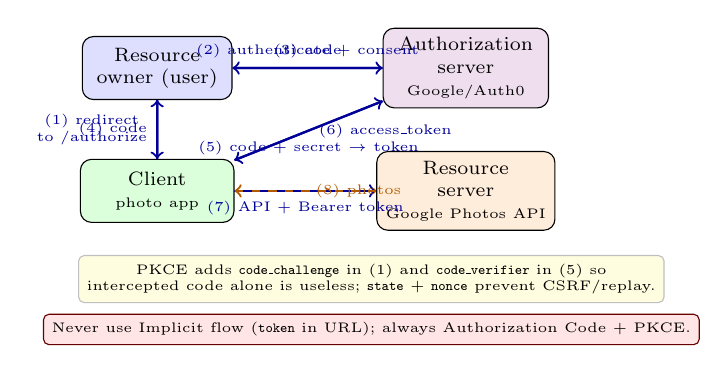
\begin{tikzpicture}[scale=0.80, every node/.style={font=\scriptsize},
  arr/.style={->,thick,blue!60!black}, darr/.style={->,thick,orange!70!black,dashed}]
  \node[draw,fill=blue!13,rounded corners=4pt,minimum width=1.9cm,minimum height=0.8cm,align=center] (user) at (-4.7,2.8) {Resource\\owner (user)};
  \node[draw,fill=green!14,rounded corners=4pt,minimum width=1.95cm,minimum height=0.8cm,align=center] (client) at (-4.7,0.85) {Client\\ \tiny photo app};
  \node[draw,fill=violet!13,rounded corners=4pt,minimum width=2.1cm,minimum height=0.8cm,align=center] (auth) at (0.2,2.8) {Authorization\\server\\ \tiny Google/Auth0};
  \node[draw,fill=orange!14,rounded corners=4pt,minimum width=2.1cm,minimum height=0.8cm,align=center] (rs) at (0.2,0.85) {Resource\\server\\ \tiny Google Photos API};
  % Flow steps
  \draw[arr] (client) -- (user) node[midway,left,font=\tiny,align=center] {(1) redirect\\to /authorize};
  \draw[arr] (user) -- (auth) node[midway,above,font=\tiny] {(2) authenticate + consent};
  \draw[arr] (auth) -- (user) node[midway,above,font=\tiny] {(3) code};
  \draw[arr] (user) -- (client) node[midway,left,font=\tiny] {(4) code};
  \draw[arr] (client) -- (auth) node[midway,below,font=\tiny] {(5) code + secret $\to$ token};
  \draw[arr] (auth) -- (client) node[midway,right,font=\tiny] {(6) access\_token};
  \draw[arr] (client) -- (rs) node[midway,below,font=\tiny] {(7) API + Bearer token};
  \draw[darr] (rs) -- (client) node[midway,right,font=\tiny] {(8) photos};
  \node[font=\tiny,fill=yellow!12,draw=gray!50,rounded corners=2pt,inner sep=3pt,align=center] at (-1.3,-0.55) {PKCE adds \texttt{code\_challenge} in (1) and \texttt{code\_verifier} in (5) so\\intercepted code alone is useless; \texttt{state} + \texttt{nonce} prevent CSRF/replay.};
  \node[font=\tiny,fill=red!10,draw=red!40!black,rounded corners=2pt,inner sep=3pt,align=center] at (-1.3,-1.35) {Never use Implicit flow (\texttt{token} in URL); always Authorization Code + PKCE.};
\end{tikzpicture}
\caption{OAuth 2.0 Authorization Code flow with PKCE (current best practice). Steps 1--4 happen via the browser redirect; steps 5--6 are a direct back-channel call with the client secret. OIDC adds an \texttt{id\_token} (JWT) in step 6 so the client learns \emph{who} logged in.}
\label{fig:oauth-flow}
\end{figure}

Key threats and fixes: \emph{authorization-code interception} is mitigated by \emph{PKCE} (the client proves it initiated the flow), \emph{CSRF} in the redirect by a random \texttt{state} value, \emph{token leakage} by keeping tokens out of URLs and storing them securely, and \emph{over-scoping} by requesting minimal scopes (\texttt{photos.read} not \texttt{photos.*}). The access token is a bearer credential---whoever holds it can call the API---so short lifetimes ($5$--$15$~min) plus refresh tokens are standard. Refresh tokens must be sender-constrained or rotated on use.

MFA, session hygiene and OAuth compose: a site that offers ``Log in with Google'' still needs its own session cookie (Fig.~\ref{fig:session-flow}) after the OAuth exchange, and should step up to MFA for sensitive actions (transfer money, delete account) even when the initial login was delegated. OIDC's \texttt{id\_token} is for identity; do not use it as an API bearer token.

% ============================================================
\section{Exercises}\label{sec:ch02-exercises}
\begin{enumerate}[label=E2.\arabic*, leftmargin=*, itemsep=0.6em]
    \item \textbf{Hashing choices.} A junior engineer proposes \texttt{SHA-256(password)} stored in the DB. Explain concretely how an attacker with a stolen table exploits this (rainbow table, GPU brute force). Then justify each of salt, slow KDF, and pepper by stating what attacker capability it removes.
    \item \textbf{Session fixation.} Describe step-by-step how an attacker can fixate a session ID (e.g., via \texttt{?SID=attackerSID}) if the server does not rotate the SID on login. Show the three HTTP exchanges (attacker, victim, attacker) and state which cookie flags would \emph{not} prevent the attack and why rotation is the correct fix.
    \item \textbf{MFA comparison.} Compare SMS OTP, TOTP (Authenticator app), and WebAuthn/FIDO2 on three axes: phishability, offline attack cost, and usability. For a university grade portal and a cryptocurrency exchange, recommend a different MFA policy for each and justify the trade-off.
    \item \textbf{OAuth threat trace.} Walk through the Authorization Code flow with PKCE (Fig.~\ref{fig:oauth-flow}) and explain at which step each of \texttt{state}, \texttt{PKCE verifier}, and short-lived tokens provides protection. Describe one concrete attack that succeeds if each is omitted.
    \item \textbf{Design task.} Design a ``change email'' flow that is safe even if the session cookie is stolen (requires current password + email OTP + re-authentication + notifying the old address). Draw a sequence diagram, choose cookie and token lifetimes, and argue why each extra step raises the cost for the attacker beyond opportunistic XSS theft.
\end{enumerate}

\section*{Chapter Notes}
OWASP Cheat Sheets for Authentication, Session Management and Forgot-Password are canonical; NIST SP 800-63B governs memorised secrets, throttling and verifier requirements. Argon2 won the 2015 Password Hashing Competition; bcrypt (Provos \& Mazi\`eres, 1999) and scrypt (Percival, 2009) remain widely deployed. For FIDO2/WebAuthn see the W3C Recommendation (2019) and CTAP spec. OAuth 2.0 is RFC~6749 (2012) with Security Best Current Practice (RFC~6819, draft-ietf-oauth-security-topics); OIDC is built on top (OpenID Foundation, 2014). PKCE is RFC~7636.
% End of Chapter 2 -- 230 lines target
